\section{Describing Roof Overhangs}\label{describing-roof-overhangs}

Building heat transfer surfaces, such as roofs and walls, only cast shadows in a hemisphere in the direction of the outward facing normal (see Figure~\ref{fig:building-heat-transfer-surfaces-cast-shadows}). Because roof surfaces generally face upward, a roof surface which extends beyond the walls of the building will not cast shadows on the walls below it (see Figure~\ref{fig:extended-roof-surface-will-not-shade}).

\begin{figure}[hbtp] % fig 3
\centering
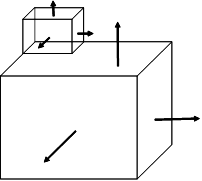
\includegraphics[width=0.9\textwidth, height=0.9\textheight, keepaspectratio=true]{media/image003.png}
\caption{Building heat transfer surfaces cast shadows in the direction of outward facing normal. \protect \label{fig:building-heat-transfer-surfaces-cast-shadows}}
\end{figure}

\begin{figure}[hbtp] % fig 4
\centering
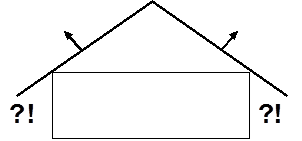
\includegraphics[width=0.9\textwidth, height=0.9\textheight, keepaspectratio=true]{media/image004.png}
\caption{Extended roof surface will not shade the walls below. \protect \label{fig:extended-roof-surface-will-not-shade}}
\end{figure}

Figure~\ref{fig:proper-surface-configurations-for-roof} shows the proper surface configurations for two types of attic construction. In all cases, the roof surface should only include the area of the roof which contacts the zone below it. In these drawings, this is an unconditioned attic space, but it could also be a conditioned zone. Any extensions of the roof which are exposed to the outdoors on both sides should be described as a shading surface.

For the configuration on the left, the overhang should be a shading surface which will cast shadows in both directions (if the default mirroring is disabled the shading surface must face downward). This ensures that the correct shading will be modeled, and it also avoids overstating the heat transfer through the roof into the attic.

For the configuration on the right, the attic is fully enclosed with building heat transfer surfaces for the roof and soffits. The soffits would be described as floor surfaces in the attic and would face downward. The central portion of the attic floor would be described as an interzone floor surface where the outside boundary condition is the ceiling surface in the zone below.

\begin{figure}[hbtp] % fig 5
\centering
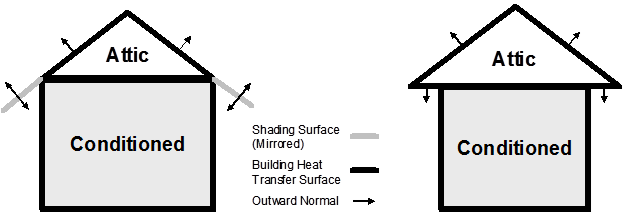
\includegraphics[width=0.9\textwidth, height=0.9\textheight, keepaspectratio=true]{media/image005.png}
\caption{Proper surface configurations for roof overhangs for two types of attic construction. \protect \label{fig:proper-surface-configurations-for-roof}}
\end{figure}
